% -------------------------------------------------------------------------------------------------------
%-----------------------------CONSULTA DE RECURSOS HUMANOS---------------------------------
% -------------------------------------------------------------------------------------------------------

\section{Gestión de Recursos Humanos}
    Para ver la lista de recursos humanos que tiene a su cargo, el Jefe de Innovación Educativa primero debe seleccionar la opción \textbf{Gestionar Recursos Humanos} del menú ubicado en la parte izquierda, así puede observar la siguiente pantalla:

        % Imagen de Consultar recursos humanos
        \begin{figure}[H]
            \centering
            \hypertarget{consultarRH}{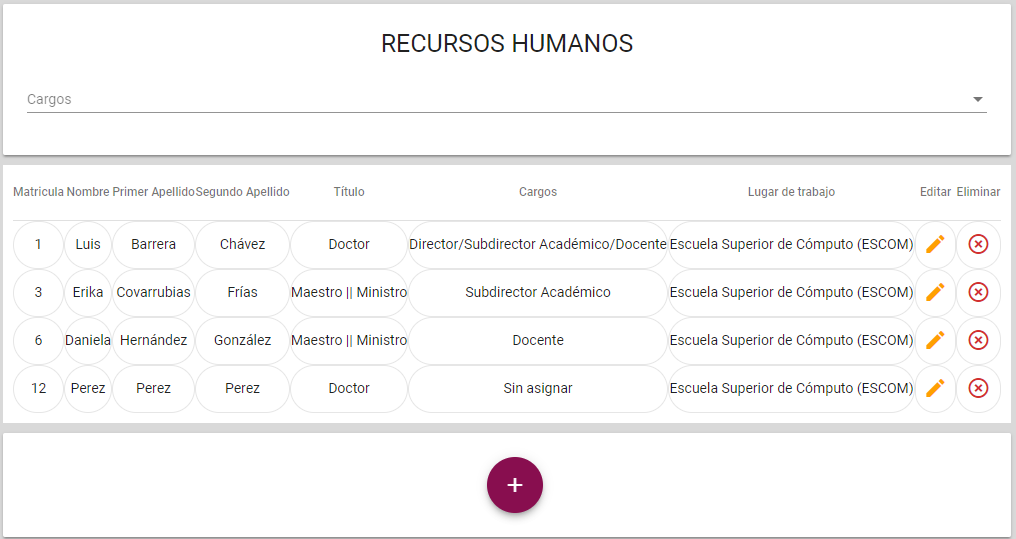
\includegraphics[width=0.7\linewidth]{images/SP1/ConsultarRH}}
            \caption{Pantalla para consultar recursos humanos}
            \label{consultarrh}
        \end{figure}

        En esa pantalla, aparecen de forma predeterminada todos los recursos humanos que el Jefe de Innovación Educativa tiene a su cargo y que están registrados en el sistema hasta el momento. El Jefe de Innovación Educativa tiene a su disposición 2 funciones:
        \newpage
        \begin{enumerate}

            \item   Buscar recursos humanos según el cargo que ocupan.

                Para esto el Jefe de Innovación Educativa tiene que seleccionar el cargo que desea consultar en el siguiente componente:

                \begin{figure}[H]
                    \centering
                    \hypertarget{cargo1}{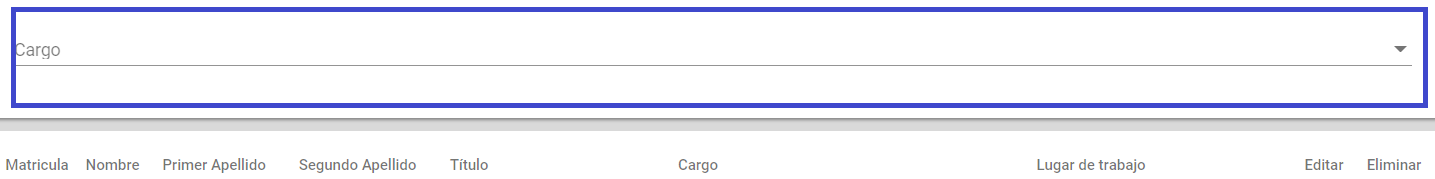
\includegraphics[width=0.7\linewidth]{images/SP1/BtnCargo1}}
                    \caption{Selección de Cargo}
                    \label{cargo1}
                \end{figure}

                 Y a continúación el sistema muestra todos los recursos humanos que tengan el cargo seleccionado.

                    \item Eliminar recursos humanos.

                Para esta última acción, el Jefe de Innovación Educativa debe dar clic en el botón con el icono de una equis en color rojo que está al lado del recurso humano que desee  eliminar.

                \begin{figure}[H]
                    \centering
                    \hypertarget{eliminar}{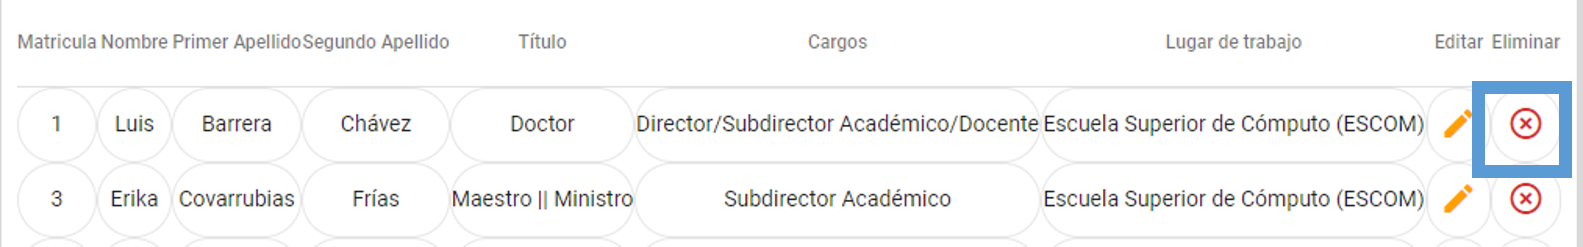
\includegraphics[width=0.7\linewidth]{images/SP1/BtnEliminar}}
                    \caption{Botón Eliminar Recursos Humanos}
                    \label{eliminar}
                \end{figure}

                Al hacer esto, el sistema despliega el siguiente mensaje:

                %Imagen del MSG22
               \begin{figure}[H]
                    \centering
                    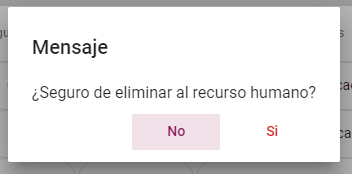
\includegraphics[width=0.4\linewidth]{images/SP1/MSG22}
                \caption{Confirmación de eliminación}
                \label{confirmarE}

                \end{figure}

                Para confirmar, el Jefe de Innovación Educativa debe dar clic en el botón “Sí”, y en ese momento el recurso humano es removido del sistema y el Jefe de Innovación Educativa permanece en la pantalla \hyperlink{consultarRH}{\textit{Consultar Recursos Humanos}}.


                Para cancelar, el Jefe de Innovación Educativa debe dar clic en botón “No”, y en ese momento el mensaje se cierra, el recurso humano no se elimina, y el Jefe de Innovación Educativa permanece en la pantalla de \hyperlink{consultarRH}{\textit{Consultar Recursos Humanos}}.



        \end{enumerate}

        También mediante botones de esta pantalla puede acceder a las siguientes 2 funciones:

        \subsubsection{Editar recursos humanos}

            Para esto, el Jefe de Innovación Educativa debe dar clic en el botón con el icono de un lápiz amarillo que está al lado del recurso humano que desea modificar. Al hacer esto el sistema muestra la pantalla   de \hyperlink{editarRH}{\textit{Editar Recurso Humano}}.

            \begin{figure}[H]
                \centering
                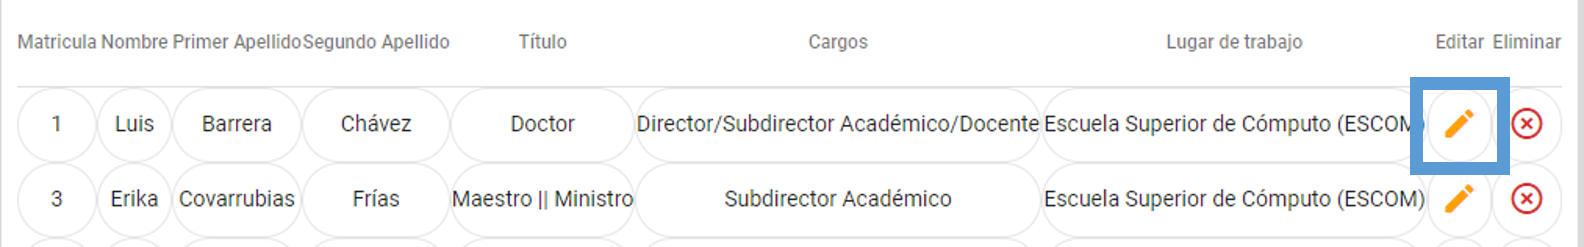
\includegraphics[width=0.7\linewidth]{images/SP1/BtnEditar}
                \caption{Botón Editar Recursos Humanos}
                \label{editar}
            \end{figure}

            Para más detalles de editar usuarios vaya a la sección \hyperlink{editar-RH}{Edición de Recursos Humanos}.

        \subsubsection{Registrar recursos humanos}

            Para esto el Jefe de Innovación Educativa tiene que dar clic en el botón “+” en la parte inferior de la pantalla. Al hacerlo, el sistema  lo redirecciona a la pantalla de \hyperlink{registrarRH}{\textit{Registrar Recurso Humano}}.

            \begin{figure}[H]
                \centering
                \hypertarget{add}{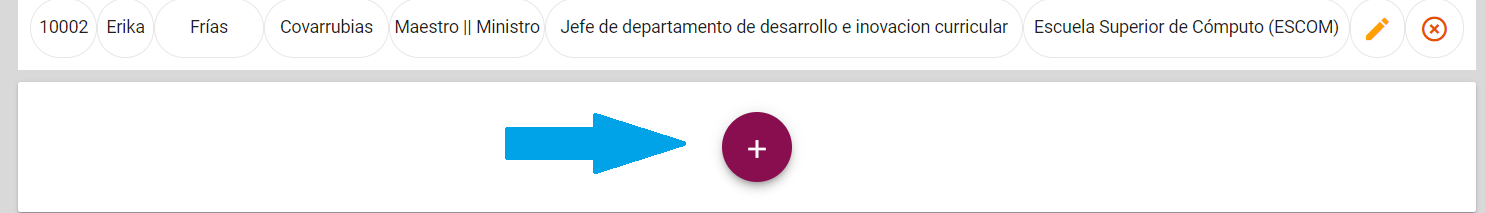
\includegraphics[width=0.7\linewidth]{images/SP1/BtnAgregar}}
                \caption{Botón Agregar Recursos Humanos}
                \label{add}
            \end{figure}

            Para más detalles de registrar recursos humanos vaya a la sección \hyperlink{registrarRH}{Registrar recurso humano}.

        \subsubsection{Posibles errores}
          \begin{itemize}
                \item Si al  presionar la opción Gestionar Recursos Humanos no se carga la información de los cargos disponibles para el Jefe de Innovación Educativa, se presenta el siguiente mensaje:

            % Imagen del MSG7
             \begin{figure}[H]
                \centering
                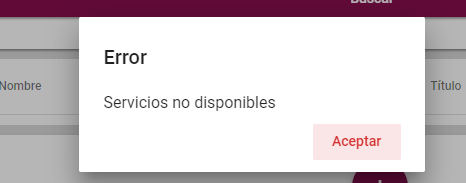
\includegraphics[width=0.4\linewidth]{images/SP1/MSGSN}
                \caption{Servicios no disponibles}
                \label{SND}

            \end{figure}

                    Al dar clic en el botón ''Aceptar'', el sistema continúa en la pantalla  \hyperlink{consultarRH}{\textit{Consultar Recursos Humanos}} y tiene que intentarlo  mas tarde.


              \item Si al intentar eliminar un recurso humano aparece el siguiente mensaje:
              % Imagen del MSG56
                \begin{figure}[H]
                   \centering
                   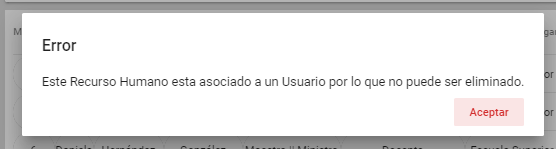
\includegraphics[width=0.4\linewidth]{images/SP1/MSG56}
                    \caption{Recurso humano asociado a un usuario no puede ser eliminado}
                   \label{mensaje56}
                \end{figure}

                Significa que ese recurso humano tiene una cuenta de usuario registrada en el sistema. Primero, el Jefe de Innovación Educativa debe de ir a la opción \textbf{Gestionar Usuarios} del menú ubicado en la parte izquierda y eliminar su cuenta de usuario.

                Para más detalles de eliminar un recurso humano registrado como usuario en el sistema vaya a la sección \hyperlink{consultarUs}{\textit{Consultar Usuarios}}.


           \end{itemize}

           %%% MENSAJE DE VINCULACION CON USUARIO


        % ------------------------------------------------------------------------------------
        % ----------------------------- REGISTRAR  USUARIOS ---------------------------------
        % ------------------------------------------------------------------------------------

    \newpage
        \hypertarget{registrarRH}{}
        \subsection{Registrar Recursos Humanos}
            Si el Jefe de Innovación Educativa  en la pantalla de \hyperlink{consultarRH}{\textit{Consultar Recursos Humanos}} da clic en el botón ''+'', aparece la siguiente pantalla:

            \begin{figure}[H]
                \centering
                \hypertarget{registrarUs}{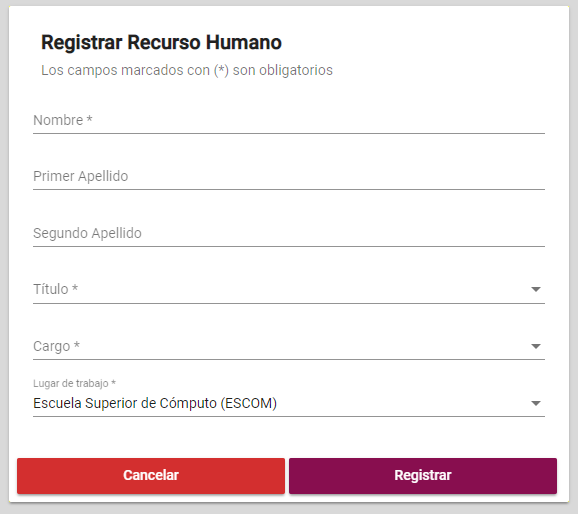
\includegraphics[width=0.7\linewidth]{images/SP1/RegistrarRH}}
                \caption{Pantalla para registrar recursos humanos}
                \label{registrarrh}
            \end{figure}

            El Jefe de Innovación Educativa tiene que ingresar la información correspondiente del nuevo recurso humano en el formulario. Un ejemplo del llenado es el siguiente:

            \begin{figure}[H]
                \centering
                \hypertarget{ejreg}{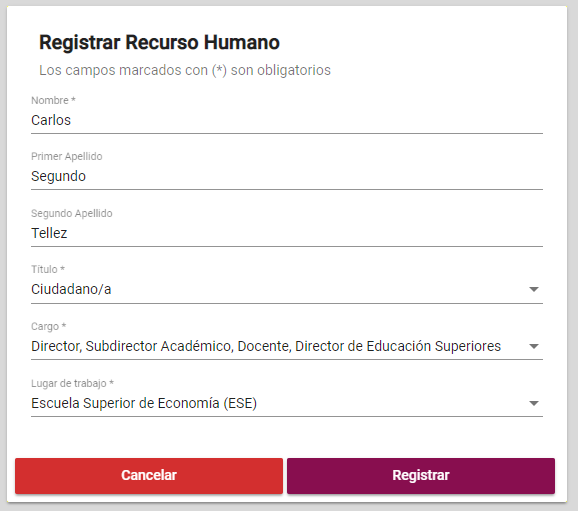
\includegraphics[width=0.7\linewidth]{images/SP1/RegistrarLleno}}
                \caption{Ejemplo de llenado para agregar un nuevo recurso humano}
                \label{ejreg}
            \end{figure}

    \newpage
            Si el Jefe de Innovación Educativa presiona el botón de “Cancelar”:

            \begin{figure}[H]
                \centering
                \hypertarget{cancel1}{
\includegraphics[width=0.7\linewidth]{images/SP1/BtnCancelar1}}
                \caption{Botón ''Cancelar''}
                \label{cancel1}
            \end{figure}

            El sistema muestra el siguiente mensaje:

            %Imagen MSG29

             \begin{figure}[H]
                \centering
            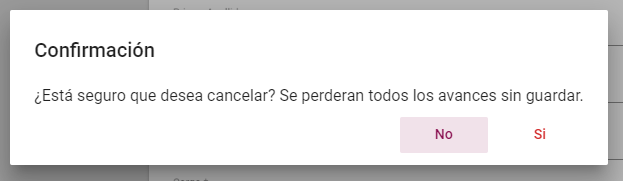
\includegraphics[width=0.4\linewidth]{images/SP1/MSG29}
                \caption{Cancelar Acción}
                \label{mensaje29}
            \end{figure}

            Para confirmar, el Jefe de Innovación Educativa tiene que dar clic en el botón “Sí”, el recurso humano no es registrado y regresa a la pantalla de \hyperlink{consultarRH}{\textit{Consultar Recursos Humanos}}.

            Para continuar con el registro, el Jefe de Innovación Educativa tiene que  dar clic el botón “No”, el mensaje se cierra y el Jefe de Innovación Educativa continúa en el formulario para terminar el registro.

            Cuando el Jefe de Innovación Educativa considere que los datos sean correctos y esten completos, debe de dar clic en el botón “Registrar”.

            \begin{figure}[H]
                \centering
                \hypertarget{btnreg}{
\includegraphics[width=0.7\linewidth]{images/SP1/BtnRegistrar}}
                \caption{Botón ''Registrar''}
                \label{btnreg}
            \end{figure}

            Si no se presentan errores el sistema muestra el mensaje:

            % Imagen MSG5

             \begin{figure}[H]
                \centering
            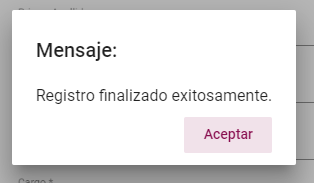
\includegraphics[width=0.4\linewidth]{images/SP1/MSG5}
                \caption{Registro exitoso}
                \label{mensaje5}

            \end{figure}

            Al dar clic en el botón “Aceptar”, el sistema muestra la pantalla de  \hyperlink{consultarRH}{\textit{Consultar Recursos Humanos}}.

            \subsubsection{Posibles errores}

                \begin{itemize}
                    \item Problemas con la conexión o el sistema

                        Si al momento de acceder a la pantalla de \hyperlink{registrarRH}{\textit{Registrar Recurso Humano}} o al intentar registrar un recurso humano, aparece el siguiente mensaje:
                        %Imagen MSG7 Y MSG25

                        \begin{figure}[H]
                        \centering
                        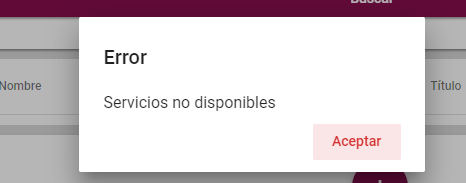
\includegraphics[width=0.4\linewidth]{images/SP1/MSGSN}
                        \caption{Servicios no disponibles}
                        \label{SND}

                      \end{figure}

                        Significa que existe un error de conexión o del sistema. Al dar clic en en botón ''Aceptar'', el sistema lo redirecciona a la pantalla de \hyperlink{consultarRH}{\textit{Consultar Recursos Humanos}}. Debe esperar a que la página este disponible para  intentar acceder nuevamente.

                    \item Campos vacíos al momento de agregar un nuevo recurso humano

                        Si el Jefe de Innovación Educativa deja en blanco algún campo o campos del formulario, y posteriormente da clic en el botón ''Registrar'', el sistema muestra el siguiente mensaje debajo del campo o campos:
                        %Imagen MSG44

                         \begin{figure}[H]
                            \centering
                        
\includegraphics[width=0.4\linewidth]{images/SP1/MSG44}
                            \caption{Campos vacíos}
                        \label{mensaje44}
                       \end{figure}

                         El Jefe de Innovación Educativa debe de dar clic en ''Aceptar'' y el sistema regresa al formulario, en donde el Jefe de Innovación Educativa debe llenar el o los campos que estan vacíos.

                    \item Los campos ingresados no son válidos

                        Si al momento de dar clic en el botón ''Registrar'' aparece el siguiente mensaje:
                        %Imagen MSG35
                             % Imagen del MSG35
                         \begin{figure}[H]
                            \centering
                            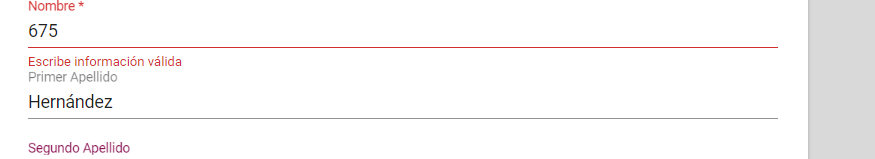
\includegraphics[width=0.4\linewidth]{images/SP1/MSG35}
                            \caption{Campos incorrectos}
                            \label{mensaje35}

                        \end{figure}

                        Significa que la composición de los datos ingresados en el formulario no es la correcta. Tenga en cuenta lo siguiente:

                        \begin{itemize}
                            \item El nombre y apellidos deben iniciar con mayúscula, puede poner más de uno por campo en caso de 2 nombres o apellidos compuestos.
                            \item El Jefe de Innovación Educativa altera la información de los selectores de cargo o zona de trabajo.
                            %\item La contraseña no acepta acentos, espacios o caracteres especiales.
                        \end{itemize}

                \end{itemize}

            % ------------------------------------------------------------------------------------
            % ------------------------------ EDICION DE USUARIOS ---------------------------------
            % ------------------------------------------------------------------------------------
\newpage

            \hypertarget{editar-RH}{}
            \subsection{Edición de Recursos Humanos}
                Si el Jefe de Innovación Educativa en la pantalla de \hyperlink{consultarRH}{\textit{Consultar Recursos Humanos}} da clic en el botón con el icono de un lápiz amarillo de un recurso humano, aparece la siguiente pantalla:

                \begin{figure}[H]
                    \centering
                    \hypertarget{editarRH}{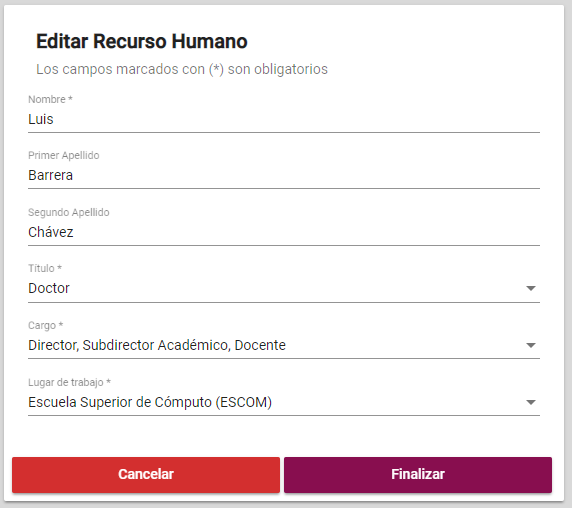
\includegraphics[width=0.6\linewidth]{images/SP1/EditarRH}}
                    \caption{Pantalla para la edición de recursos humanos}
                    \label{editarrh}
                \end{figure}

                En esta pantalla se cargan los datos del recurso humano correspondiente por el lápiz amarillo seleccionado en la pantalla de \hyperlink{consultarRH}{\textit{Consultar Recursos Humanos}} y llena el formulario.

                A continuación, el Jefe de Innovación Educativa puede modificar todos los campos del recurso humano.

                Si el Jefe de Innovación Educativa presiona el botón de “Cancelar”:

                \begin{figure}[H]
                    \centering
                    \hypertarget{cancel2}{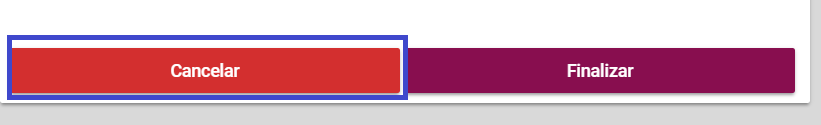
\includegraphics[width=0.7\linewidth]{images/SP1/BtnCancelar2}}
                    \caption{Botón ''Cancelar''}
                    \label{cancel2}
                \end{figure}

                El sistema muestra el siguiente mensaje:
                %Imagen MSG29
                  \clearpage
                 \begin{figure}[H]
                    \centering
                    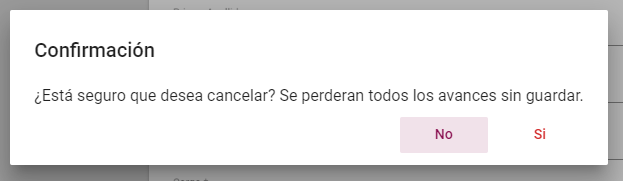
\includegraphics[width=0.4\linewidth]{images/SP1/MSG29}
                    \caption{Cancelar cambios}
                    \label{mensaje29}

                \end{figure}

                Para confirmar, el Jefe de Innovación Educativa tiene que dar clic en el botón “Sí”, los datos del recurso humano no son modificados  y regresa a la pantalla \hyperlink{consultarRH}{\textit{Consultar Recursos Humanos}}

                Para continuar con la modificación, el Jefe de Innovación Educativa tiene que  dar clic el botón “No”, el mensaje se cierra y el Jefe de Innovación Educativa continúa en el formulario para terminar la modificación.

                Cuando el Jefe de Innovación Educativa considere que los datos son correctos y están completos, debe de dar clic en el botón “Finalizar”.
                \begin{figure}[H]
                    \centering
                    \hypertarget{btnfin}{
\includegraphics[width=0.7\linewidth]{images/SP1/BtnFinalizar}}
                    \caption{Botón ''Finalizar''}
                    \label{btnfin}
                \end{figure}

                Si no se presentan errores el sistema muestra el mensaje:
                %Imagen MSG31

                 \begin{figure}[H]
                    \centering
                    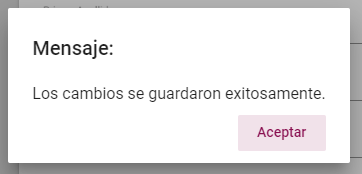
\includegraphics[width=0.4\linewidth]{images/SP1/MSG31}
                    \caption{Cambios guardados}
                    \label{mensaje31}

                \end{figure}

                Al dar clic en el botón “Aceptar”, el sistema muestra la pantalla de \hyperlink{consultarRH}{\textit{Consultar Recursos Humanos}}.

                \subsubsection{Posibles errores}
                    \begin{itemize}
                        \item Problemas con la conexión o el sistema

                            Si al momento de acceder a la pantalla de \hyperlink{editarRH}{\textit{Editar Recurso Humano}} o al intentar modificar un recurso humano, aparece el siguiente mensaje:
                            \clearpage
                            \begin{figure}[H]
                                \centering
                                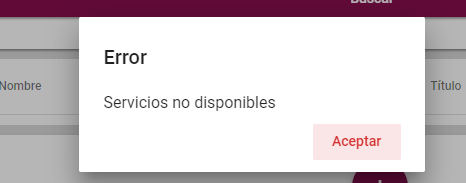
\includegraphics[width=0.4\linewidth]{images/SP1/MSGSN}
                                \caption{Servicios no disponibles}

                            \end{figure}


                            Significa que existe un error de conexión o del sistema. Al dar clic en en botón ''Aceptar'', el sistema redirecciona al Jefe de Innovación Educativa a la pantalla de \hyperlink{consultarRH}{\textit{Consultar Recursos Humanos}}. El Jefe de Innovación Educativa debe esperar a que la página este disponible para intentar acceder nuevamente.

                        \item Campos vacíos al momento de modificar al usuario

                            Si el Jefe de Innovación Educativa deja en blanco algún campo o campos del formulario, y posteriormente da clic en el botón ''Finalizar'', el sistema muestra el siguiente mensaje debajo del campo o campos:
                           %Imagen MSG3X

                          \begin{figure}[H]
                            \centering
                            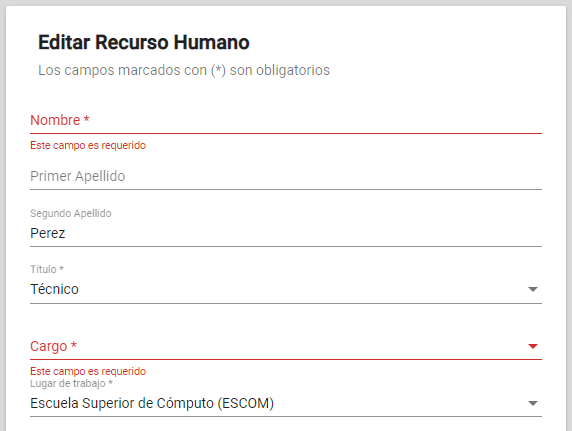
\includegraphics[width=0.4\linewidth]{images/SP1/MSG44-1}
                            \caption{Campos vacíos}
                            \label{mensaje44}

                         \end{figure}

                           El Jefe de Innovación Educativa regresa al formulario, en donde debe llenar el o los campos que estan vacíos.

                        \item Los campos ingresados no son válidos

                            Si al momento de dar clic en el botón ''Finalizar'' aparece el siguiente mensaje:
                            \clearpage
                                \begin{figure}[H]
                            \centering
                            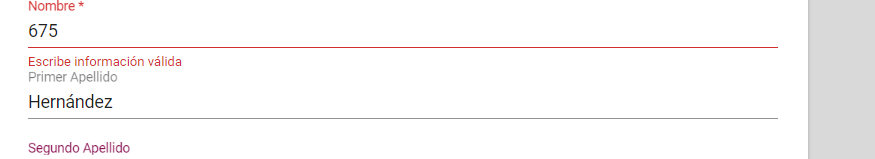
\includegraphics[width=0.4\linewidth]{images/SP1/MSG35}
                            \caption{Campos incorrectos}
                            \label{mensaje35}

                         \end{figure}


                            Significa que la composición de los datos ingresados en el formulario no es la correcta. Tenga en cuenta lo siguiente:

                            \begin{itemize}
                                \item El nombre y apellidos deben iniciar con mayúscula, puede poner más de uno por campo en caso de 2 nombres o apellidos compuestos.
                                \item El Jefe de Innovación Educativa altera la información de los selectores de cargo o zona de trabajo.
                            \end{itemize}



                    \end{itemize}